\section{函数解析的充要条件}

\subsection{柯西-黎曼方程}
\begin{frame}{可导函数的特点}
	\onslide<+->
	通过对一些简单函数的分析, 我们会发现可导的函数往往可以直接表达为 $z$ 的函数的形式, 而不解析的往往包含 $x,y,\ov z$ 等内容.
	\onslide<+->
	这种现象并不是孤立的.
	\onslide<+->
	我们来研究二元实变量函数的可微性与复变函数可导的关系.

	\onslide<+->
	为了简便我们用 $u_x,u_y,v_x,v_y$ 等记号表示偏导数.
\end{frame}


\begin{frame}{可导的等价刻画: 形式推导}
	\onslide<+->
	设 \alert{$f$ 在 $z$ 处可导}, $f'(z)=a+bi$,
	\onslide<+->
	则
	\[\Delta u+i\Delta v=\Delta f=(a+bi)(\Delta x+i\Delta y)+o(\Delta z).\]
	\onslide<+->展开可知
	\begin{align*}
		\Delta u&=a\Delta x-b\Delta y+o(\Delta z),\\
		\Delta v&=b\Delta x+a\Delta y+o(\Delta z).
	\end{align*}
	\onslide<+->
	由于 $o(\Delta z)=o(|\Delta z|)=o(\sqrt{x^2+y^2})$,
	\onslide<+->
	因此 \alert{$u,v$ 可微且 $u_x=v_y=a,v_x=-u_y=b$}.
\end{frame}


\begin{frame}{可导的等价刻画: 形式推导}
	\onslide<+->
	反过来, 假设 \alert{$u,v$ 可微且 $u_x=v_y, v_x=-u_y$}.
	\onslide<+->
	由全微分公式
	\begin{align*}
		\Delta u&=u_x\Delta x+u_y\Delta y+o(\Delta z)
			=u_x\Delta x-v_x\Delta y+o(\Delta z),\\
			\visible<+->{\Delta v}&\visible<.->{=v_x\Delta x+v_y\Delta y+o(\Delta z)
			=v_x\Delta x+u_x\Delta y+o(\Delta z),}\\
		\visible<+->{\Delta f}&
		\visible<.->{=\Delta (u+iv)=(u_x+i v_x)\Delta x+(-v_x+i u_x)\Delta y}+o(\Delta z)\\
		&\visible<+->{=(u_x+i v_x)\Delta(x+iy)+o(\Delta z)}\\
		&\visible<+->{=(u_x+i v_x)\Delta z+o(\Delta z).}
	\end{align*}
	\onslide<+->
	故 \alert{$f(z)$ 在 $z$ 处可导, 且 $f'(z)=u_x+i v_x=v_y-i u_y$}.
\end{frame}


\begin{frame}{可导的等价刻画: 柯西-黎曼方程}
	\onslide<+->
	由此得到
	\onslide<+->
	\begin{algorithm}{柯西-黎曼定理}
		$f(z)$ 在 $z$ 可导当且仅当在 $z$ 点 $u,v$ 可微且满足柯西-黎曼方程 (简称为 C-R 方程):
		\[u_x=v_y,\quad v_x=-u_y.\]
		此时
		\[f'(z)=u_x+iv_x=v_y-iu_y.\]
	\end{algorithm}

	\onslide<+->
	\begin{center}
		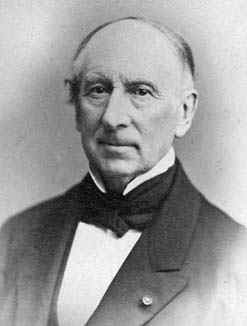
\includegraphics[height=25mm]{../image/Cauchy.jpeg}
		\hspace{2cm}
		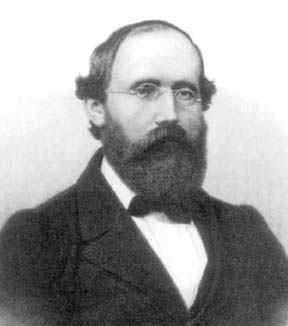
\includegraphics[height=25mm]{../image/Riemann.jpeg}
	\end{center}
\end{frame}


\begin{frame}{柯西-黎曼方程的等价形式\noexer}
	\onslide<+->
	注意到 $x=\dfrac12z+\dfrac12\ov z,y=-\dfrac i2z+\dfrac i2\ov z$.
	\onslide<+->
	仿照着二元实函数偏导数在变量替换下的变换规则, 我们定义 $f$ 对 $z$ 和 $\ov z$ 的偏导数为
	\[\laeq{\displaystyle
		\pp fz=\pp xz\pp fx+\pp yz\pp fy
		=\frac12\pp fx-\frac i2\pp fy,\\
		\displaystyle
		\pp f{\ov z}=\pp x{\ov z}\pp fx+\pp y{\ov z}\pp fy
		=\frac12\pp fx+\frac i2\pp fy.
	}.\]
	\onslide<+->
	如果把 $z,\ov z$ 看成独立变量, 那么当 $f$ 在 $z$ 处可导时,
	$\diff f=f'\diff z$.
	当 $f$ 关于 $z,\ov z$ 可微时(即 $u,v$ 可微),
	\[\diff f=\pp fz\diff z+\pp f{\ov z}\diff\ov z.\]
	\onslide<+->
	所以 \alert{$f$ 在 $z$ 处可导当且仅当 $u,v$ 可微且 $\dpp f{\ov z}=0$, 此时 $f'(z)=\dpp fz$.}
\end{frame}


\begin{frame}{可导的充分性条件}
	\onslide<+->
	由于二元函数的偏导数均连续蕴含可微, 因此我们有:

	\onslide<+->
	\begin{theorem}
		\begin{itemize}
			\item 如果 $u_x,u_y,v_x,v_y$ 在 $z$ 处连续, 且满足C-R方程, 则 $f(z)$ 在 $z$ 可导.
			\item 如果 $u_x,u_y,v_x,v_y$ 在区域 $D$ 上处处连续, 且满足C-R方程, 则 $f(z)$ 在 $D$ 上可导(从而解析).
		\end{itemize}
	\end{theorem}
\end{frame}


\subsection{柯西-黎曼方程的应用}
\begin{frame}{典型例题: 利用C-R方程判断可导和解析}
	\onslide<+->
	\begin{example}
		函数 $f(z)=\ov z$ 在何处可导, 在何处解析?
	\end{example}

	\onslide<+->
	\begin{solution}
		由 $u=x,v=-y$ 可知
		\begin{align*}
			u_x&=1,&u_y&=0,\\
			v_x&=0,&v_y&=-1.
		\end{align*}
		\onslide<+->{%
			因为 $u_x=1\neq v_y=-1$, 所以该函数处处不可导, 处处不解析.
		}
	\end{solution}
	\onslide<+->
	也可由 $\dpp f{\ov z}=1\neq0$ 看出.
\end{frame}


\begin{frame}{典型例题: 利用C-R方程判断可导和解析}
	\onslide<+->
	\begin{example}
		函数 $f(z)=z\Re z$ 在何处可导, 在何处解析?
	\end{example}

	\onslide<+->
	\begin{solution}
		由 $f(z)=x^2+ixy,u=x^2,v=xy$
		\onslide<+->{%
			可知
			\begin{align*}
				u_x&=2x,&u_y&=0,\\
				v_x&=y, &v_y&=x.
			\end{align*}
		}\onslide<+->{%
			由 $2x=x,0=-y$ 可知只有 $x=y=0,z=0$ 满足C-R方程.
		}\onslide<+->{%
			因此该函数只在 $0$ 可导, 处处不解析且
			\[f'(0)=u_x(0)+iv_x(0)=0.\]
		}
		\vspace{-\baselineskip}
	\end{solution}
	\onslide<+->
	也可由 $f=\dfrac12 z(z+\ov z), \dpp f{\ov z}=\dfrac12 z$ 看出, $f'(0)=\dpp fz\Big|_{z=0}=z|_{z=0}=0$.
\end{frame}


\begin{frame}{典型例题: 利用C-R方程判断可导和解析}
	\onslide<+->
	\begin{example}
		函数 $f(z)=e^x(\cos y+i\sin y)$ 在何处可导, 在何处解析?
	\end{example}

	\onslide<+->
	\begin{solution}
		由 $u=e^x\cos y,v=e^x\sin y$
		\onslide<+->{%
			可知
			\begin{align*}
			u_x&=e^x\cos y,&u_y&=-e^x\sin y,\\
			v_x&=e^x\sin y,&v_y&=e^x\cos y.
			\end{align*}
		}\onslide<+->{%
			因此该函数处处可导, 处处解析, 且
			\[f'(z)=u_x+iv_x=e^x(\cos y+i\sin y)=f(z).\]
		}
	\vspace{-\baselineskip}
	\end{solution}

	\onslide<+->
	实际上, 这个函数就是复变量的指数函数 $e^z$.
\end{frame}


\begin{frame}{典型例题: 利用C-R方程判断可导和解析}
	\onslide<+->
	\begin{exercise}
		函数\fillbraceframe{A}在 $z=0$ 处不可导.
		\begin{exchoice}(2)
			() $2x+3yi$
			() $2x^2+3y^2i$
			() $e^x\cos y+i e^x\sin y$
			() $x^2-xyi$
		\end{exchoice}
	\end{exercise}

	\onslide<+->
	\begin{answer}
		根据C-R方程可知对于A, $u_x(0)=2\neq v_y(0)=3$.
		\onslide<+->{对于BD, 各个偏导数在 $0$ 处取值都是 $0$.
		}\onslide<+->{C则是处处都可导.}
	\end{answer}
\end{frame}


\begin{frame}{例: 利用C-R方程判断可导和解析}
	\onslide<+->
	\begin{example}
		设函数 $f(z)=(x^2+axy+by^2)+i(cx^2+dxy+y^2)$ 在复平面内处处解析. 求实常数 $a,b,c,d$ 以及 $f'(z)$.
	\end{example}

	\onslide<+->
	\begin{solution}
		由于
		\vspace{-\baselineskip}
		\begin{align*}
			u_x&=2x+ay,&u_y=ax+2by,\\
			v_x&=2cx+dy,&v_y=dx+2y,
		\end{align*}
		\onslide<+->{因此
			\[2x+ay=dx+2y,\quad ax+2by=-(2cx+dy),\]}
		\vspace{-\baselineskip}
		\onslide<+->{
			\[a=d=2,\quad b=c=-1,\]}
		\vspace{-\baselineskip}
		\onslide<+->{
			\[f'(z)=u_x+iv_x=2x+2y+i(-2x+2y)=(2-2i)z.\]}
		\vspace{-\baselineskip}
	\end{solution}
\end{frame}


\begin{frame}[<*>]{例: 利用C-R方程证明解析函数结论}
	\onslide<+->
	\begin{example}
		如果 $f'(z)$ 在区域 $D$ 内处处为零, 则 $f(z)$ 在 $D$ 内是一常数.
	\end{example}

	\onslide<+->
	\begin{proof}
		由于 $f'(z)=u_x+iv_x=v_y-iu_y=0$,
		\onslide<+->{%
			因此 $u_x=v_x=u_y=v_y=0$, $u,v$ 均为常数,
		}\onslide<+->{%
			从而 $f(z)=u+iv$ 是常数.\qedhere
		}
	\end{proof}

	\onslide<+->
	类似地可以证明, 若 $f(z)$ 在 $D$ 内解析, 则下述条件均可推出 $f(z)$ 是常数:
	\onslide<+->
	\begin{figure}[hbpt]
		\begin{minipage}{0.48\textwidth}
			\begin{itemize}
				\item $f'(z)=0$,
				\item $|f(z)|$ 是一常数,
				\item $\arg{f(z)}$ 是一常数,
			\end{itemize}
		\end{minipage}
		\begin{minipage}{0.48\textwidth}
			\begin{itemize}
				\item $\Re{f(z)}$ 是一常数,
				\item $\Im{f(z)}$ 是一常数,
				\item $v=u^2$.
			\end{itemize}
		\end{minipage}
	\end{figure}
\end{frame}


\begin{frame}{例: 解析函数的保角性\noexer}
	\beqskip{3pt}
	\onslide<+->
	\begin{example}
		如果 $f(z)$ 解析且 $f'(z)$ 处处非零, 则曲线族 $u(x,y)=c_1$ 和曲线族 $v(x,y)=c_2$ 互相正交.
	\end{example}

	\onslide<+->
	\begin{proof*}
		由于 $f'(z)=u_x-iu_y$, 因此 $u_x,u_y$ 不全为零.
		\onslide<+->{%
			对 $u(x,y)=c_1$ 使用隐函数求导法则得 $u_x\diff x+u_y\diff y=0$,
		}\onslide<+->{%
			从而 $(u_y,-u_x)$ 是该曲线在 $z$ 处的非零切向量.
		}

		\onslide<+->{%
			同理 $(v_y,-v_x)$ 是 $v(x,y)=c_2$ 在 $z$ 处的非零切向量.
		}\onslide<+->{%
			由于
			\[u_yv_y+u_xv_x=u_yu_x-u_xu_y=0,\]
		}\onslide<+->{%
			因此二者正交.\qedhere
		}
	\end{proof*}

	\onslide<+->
	当 $f'(z_0)\neq 0$ 时, 
	\onslide<+->
	经过 $z_0$ 的两条曲线 $C_1,C_2$ 的夹角和它们的像 $f(C_1),f(C_2)$ 在 $f(z_0)$ 处的夹角总是相同的.
	\onslide<+->
	这种性质被称为\emph{保角性}.
	\onslide<+->
	这是因为 $\diff f=f'(z_0)\diff z$.
	\onslide<+->
	局部来看 $f$ 把 $z_0$ 附近的点以 $z_0$ 为中心放缩 $f'(z_0)$ 倍并逆时针旋转 $\arg{f'(z_0)}$.
	\onslide<+->
	由 $w$ 复平面上曲线族 $u=c_1,v=c_2$ 正交可知上述例题成立.
	\endgroup
\end{frame}


\begin{frame}{复变函数在实变函数导数的应用\noexer}
	\onslide<+->
	最后我们来看复数在求导中的一个应用.
	\onslide<+->
	\begin{example}
		设 $f(z)=\dfrac1{1+z^2}$, 则它在除 $z=\pm i$ 外处处解析.
		\onslide<+->{%
			当 $z=x$ 为实数时,
		}\onslide<+->{%
			\begin{align*}
			\left(\dfrac1{1+x^2}\right)^{(n)}&=f^{(n)}(x)=\frac i2\left[\frac1{x+i}-\frac1{x-i}\right]^{(n)}\\
			&\visible<+->{=\frac i2\cdot(-1)^n n!\left[\frac1{(x+i)^{n+1}}-\frac1{(x-i)^{n+1}}\right]}\\
			&\visible<+->{=(-1)^{n+1}n!\Im\frac1{(x+i)^{n+1}}}\\
			&\visible<+->{=\frac{(-1)^nn!\sin[(n+1)\arccot x]}{(x^2+1)^{\frac{n+1}2}}.}
			\end{align*}}
			\vspace{-\baselineskip}
	\end{example}
	\onslide<+->
	任意有理函数的高阶导数均可按此法计算.
\end{frame}

